
\begin{figure}
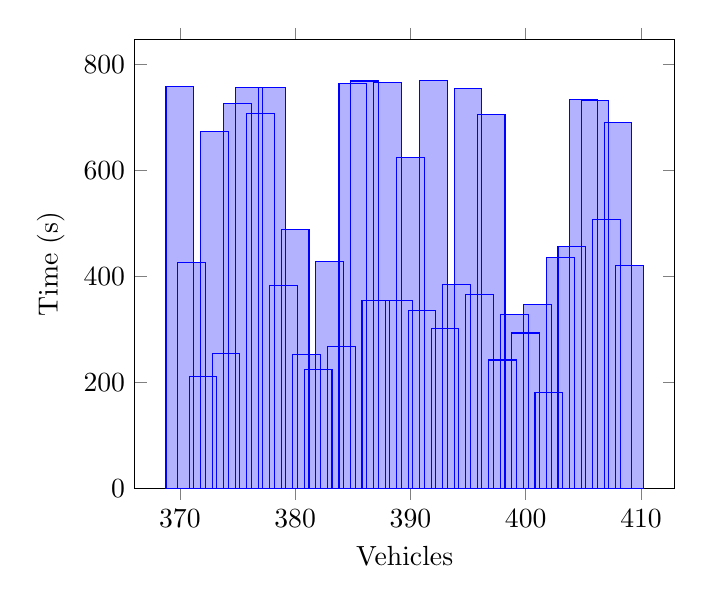
\begin{tikzpicture}
\begin{axis}[
legend style={anchor=west},
xlabel=Vehicles,
ylabel=Time (s),
ymin=0,
ybar,
]
\addplot coordinates {
(386, 769)
(392, 770)
(382, 224)
(370, 759)
(405, 734)
(409, 420)
(388, 767)
(403, 435)
(394, 384)
(391, 336)
(385, 764)
(383, 428)
(390, 624)
(389, 355)
(393, 301)
(373, 674)
(387, 354)
(374, 255)
(402, 180)
(384, 268)
(399, 328)
(397, 706)
(408, 690)
(371, 426)
(372, 211)
(401, 347)
(378, 756)
(380, 489)
(398, 242)
(376, 756)
(407, 507)
(375, 726)
(379, 383)
(404, 457)
(377, 708)
(400, 293)
(396, 365)
(406, 732)
(381, 252)
(395, 755)
};

\end{axis}
\end{tikzpicture}
\label{tik:time:0:57}
\caption{0 percent diving with GSC on route $57$}
\end{figure}
